\documentclass[a4paper]{article}
\usepackage[utf8]{inputenc}
\usepackage[T1]{fontenc}
\usepackage{amsmath, amsfonts, amssymb}
\usepackage[ruled]{algorithm2e}

\usepackage{caption}

\usepackage{graphicx}
\usepackage{float}

\usepackage[left=3cm,right=3cm,top=3cm,bottom=2cm]{geometry}

\DeclareMathOperator*{\argmin}{arg\,min}

\newcommand{\norm}[1]{\left\lVert#1\right\rVert}


\title{Approximate inference on the Ising grid}
\author{Ilyes KHEMAKHEM - Remi LE PRIOL - Brahim Khalil ABID}
\date{January 2017}
\begin{document}

\maketitle

\section{Introduction}

    The Ising model is a very important model from statistical physics used to represent multi-particle systems with interactions. It is also a classical example of a probabilistic graphical model. We consider a 2D grid $G=(V,E)$, and we suppose that each random variable $X_s$ attached to node $s$ is Bernoulli, taking values in ${-1, +1}$. Those values may represent the spin of particles in the context of physics, or the colour of a pixel in image processing. Random variables $X_s$ and $X_t$ are allowed to interact directly only if they are joined by an edge, and the energy of their interactions is $-\frac{1}{2}a_{s,t}x_sx_t$. Thus, the probability for a certain configuration $X$ is proportional to $exp(-E(x))$ where:
    \begin{equation*}
    	E(x) = -\frac{1}{2} \sum_s b_sx_s - \frac{1}{2} \sum_{s,t}a_{s,t}x_sx_t
	\label{eq:energy}
    \end{equation*}
    
    \begin{equation*}
    	\mathrm{P}(X) \propto exp(-E(x))
	\label{eq:energy2}
    \end{equation*}
$a_{s,t}$ encodes the correlation between adjacent nodes. A large $a_{s,t}$ means that $X_s$ and $X_t$ will tend to have the
same sign. $b_s$ encodes the potential at each node. $b_s > 0$ means that $X_s$ will tend to be equal to $+1$, whereas $b_s < 0$ means that $X_s$ will tend to be equal to $-1$.
In the following $\sigma$ will stand for the logistic function: $\sigma (z) = \frac{1}{1+e^{-z}}.$
\\
We consider the problem where the parameters $\theta = (a,b)$ are known. We would like to sample according to this distribution, infer the marginal probabilities, or equivalently the mean parameters $\mu = \mathbb{E}[X]$. In order to do so, we present three different algorithms in the next section, which we implemented in the particular case of an Ising grid, and compared to each other. Our work is based on \cite{a1} and \cite{b1}.

\begin{figure}[h]
	\centering
	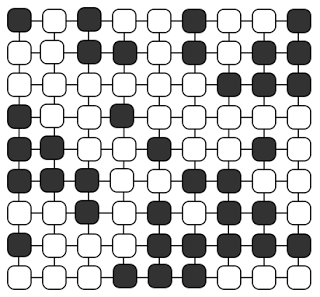
\includegraphics[scale=0.65]{rgising1}
	\caption{Example of an Ising grid}
    \label{grid}
\end{figure}

\section{Algorithms}

    The problem of inference in graphs is not easy in the general case. We have an exact algorithm, the junction tree algorithm, that works on all triangulated undirected graphs, and consequently also on directed graphs via the procedures of moralization and triangulation. However, these procedures are quite heavy, and for complex graphs the computation costs grow exponentially with the size of the maximal clique in the graph. In our work we discuss algorithms for approximate inference that would be computationally more efficient. We will present the Gibbs algorithm for sampling, and the mean field and loopy belief algorithms for inference.
    
\subsection{Gibbs sampling}
    % talk about gibbs sampling in general, 
    Starting from an initial observation, Gibbs sampling allows us to sample from the initial probability $p(X)$ by considering the Markov property so that $\mathbb{P}(X_i=.|X_{-i}=x_{-i}) = \mathbb{P}(X_i=.|X_{N_i}=x_{N_i})$, where $N_i$ is the Markov blanket of node $i$. Based on this, Gibbs sampling is an iterative algorithm that converges to the distribution $\mathrm{P}$.
    \paragraph{}
    
    % derive the precise formulation for our example,

    In the case of an Ising grid, the probability $\mathrm{P}$ takes a simple form:
        

    \begin{equation*}
        \mathbb{P}(X_i = 1 \mid X_{N_i}=x_{N_i}) = \sigma(b_i + \sum_{j \in N_i} a_{ij}x_j)
    \end{equation*}
    
    % describe the block update
    \paragraph{}
    Gibbs sampling updates can be done in multiple way. An efficient way is to sample an entire block of nodes at each iteration. In our example, we consider a checkerboard pattern, and at each iteration update half the grid.
    
    % describe the algorithm,
    \begin{algorithm}
        \caption{Checkerboard Gibbs sampling}
        \label{algo:gibbs}
        \SetKwInOut{initialization}{initialization}
        \SetKwInOut{return}{return}
        \initialization{$t = 0$ and $x^0$}
        \While{$t<T$} {
            \eIf{$t$ mod $2 == 0$}{
                {
                    B = \{first half of the checkerboard\}\;
                }
            }{
                {
                    B = \{second half of the checkerboard\}\;
                } 
            }
            {
                $\forall$ node $i \in B, x_i^t \sim Bernoulli(\sigma(b_i + \sum_{j \in N_i} a_{ij}x_j^{t-1}))$\;
            }
            {
                $x_{-B}^t = x_{-B}^{t-1}$\;
            }
        

            {
                $t=t+1$\;
            }
        }
        \return{$x^T$}

    \end{algorithm}

    % Using gibbs sampling to do inference
    \paragraph{}
    Although Gibbs sampling is used to sample observations from a graphical model, it can also be used as an inference algorithm. To compute the mean parameter $\mu = \mathbb{E}[X]$, we just execute the algorithm on the grid for multiple trajectories, and use the empirical mean to approximate $\mu$.
    
\subsection{Mean field algorithm}
    % talk about mean field in general,
    The mean field algorithm comes from field theory. The main idea behind it is that each particle feels in average the mean of the interactions with its neighbours. The validity of this approximation comes from the Law of Large Numbers, so this approximation is more efficient on dense graphs.
    
    \paragraph{}
    
    Unlike the Gibbs algorithm which is for sampling, the mean field algorithm is used to infer the mean parameters. So instead of sampling iteratively a group $X_B$ of nodes using the values of their Markov Blanket, we instead try to compute directly the mean parameters of the model. To approximate these, we compute the product model (empty graph) best approximating our model with regard to the Kullback-Leibler divergence. By doing this we get the update formula.
    % describe the algorithm, 
        \begin{algorithm}
        \SetKwInOut{initialization}{initialization}
        \SetKwInOut{return}{return}
        \initialization{$t = 0$ and $m^0$ }
        \While{$t<T$} {
            {
            $\mu_i^{t+1} = 2*\sigma( b_i + \sum\limits_{j \in N(i)} a_{i,j}\mu_j^t ) - 1 $
            }
        }
        \return{$\mu^T$}
	
        \caption{Mean field algorithm}
        \label{algo:meanfield}
    \end{algorithm}
    
    Given the update formula obtained, the mean field problem is non convex. The fixed point depends on the initialization and consequently we could obtain very different results from different initialization methods.

    % derive the precise formulation for our example,
\subsection{Loopy belief algorithm}
    % present the algorithm,
    % remind that it is exact in the case of trees,
    The sum-product message passing (or belief propagation) algorithm is a well known algorithm for exact inference on trees. It relies on the concept of messages, real valued functions passed through the edges of the graph. However, for graphs with cycles, there is no theoretical proof that this algorithm works, but we can still write it from an algorithmic point of view. For obvious reasons, it is then called loopy belief propagation.
    
    \begin{figure}[h]
    	\centering
    	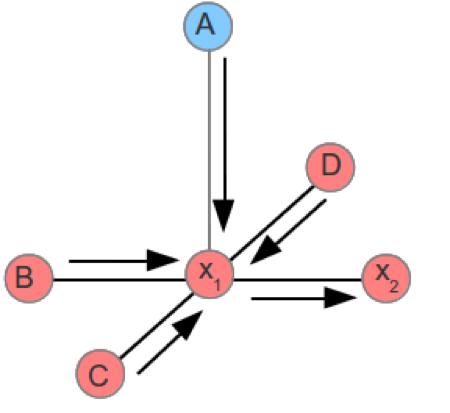
\includegraphics[scale=0.65]{messages}
    	\caption{Message passing from $x_1$ to $x_2$ with potential A and neighbors B, C and D}
        \label{messages}
    \end{figure}
    
        
    The loopy belief algorithm consists in computing iteratively the messages until convergence, and then use the final values to compute the mean parameters. The updating formula is the following:
        \begin{equation}
            m_{j \rightarrow i} (x_i) = \sum\limits_{x_j} \psi_j(x_j)\psi_{j,i}(x_i,x_j)  \   \prod\limits_{k \in N(j)\backslash \{i\} } m_{k \rightarrow j} (x_j)
            \label{message_formula}
        \end{equation}
    
    Since we have no theoretical guarantees that this algorithm converges, we had to use some tricks to make it work in the loopy case. For instance, we do not update the messages with the formula \ref{message_formula}, but we add a damping coefficient to partly keep the old messages. We also have to normalize the messages after each update to keep the messages bounded in value. Moreover, the update order can be done in more than one way: we can either update the four direction in order or choose randomly a direction to update it (while making sure we are updating all the direction equally in frequency).
    

    
    
    
    
    % describe the precise updates for our example, 
        \begin{algorithm}[h]
        \SetKwInOut{initialization}{initialization}
        \SetKwInOut{return}{return}
        \initialization{$t = 0$ and $m_{i \rightarrow j}^0$ (messages)}
        \While{$t<T$ \text{and for each direction (up, down, left, right)}} {
            
                {
                Update messages in the given direction, with a damping coefficient d:
                }
                
                {
                \begin{equation}
                 m_{j \rightarrow i}^{(t+1)_0} (x_i) = d * (\sum\limits_{x_j} \psi_j(x_j)\psi_{j,i}(x_i,x_j)  \   \prod\limits_{k \in N(j)\backslash \{i\} } m_{k \rightarrow j}^{(t+1)_0} (x_j) ) + (1-d)*m_{j \rightarrow i}^{t} (x_i)
                 \end{equation}
                
                }
                
                {
                Normalize the messages in the given direction:
                $m_{i \rightarrow j}^{t+1} (x_j) = m_{i \rightarrow j}^{(t+1)_0} (x_j) /( m_{i \rightarrow j}^{(t+1)_0} (1) + m_{i \rightarrow j}^{(t+1)_0} (-1))$
                }
                
            
        }
        \return{$m_{i \rightarrow j}^T$}

        \caption{Loopy belief algorithm with damping}
    	\label{algo:loopybelief}
    \end{algorithm}
    % describe how it was implemented (cyclic direction, batch update?)

 
%\newpage
    
\section{Experiments}
    We tested the 3 algorithms for different parameters and observations. 
    \paragraph{}
    For this section, if no index is provided for parameters $a$ and $b$, it means that these parameters are constant over the grid.
    \\
    The colour code for the figures is as follows: 
    \begin{itemize}
        \item $+1$: white or green.
        \item $-1$: black or dark blue.
        \item $0$: grey or turquoise.
    \end{itemize}
    
    % show examples of convergence for each algorithm,
    \subsection{Gibbs sampling}
    To test Gibbs sampling, we fix the potentials to 0 at each node ($b_i = 0 \forall i \in V$), and varied the initial percentage of +1 spins. We then plotted the final state of the grid for different values of the correlations $a = {-1, 0, 0.7, 0.8, 0.9, 1, 2}$ to observe the phase transition. Figure \ref{figure:gibbs} shows the result.
    
    \begin{figure}[h]
        \centering
        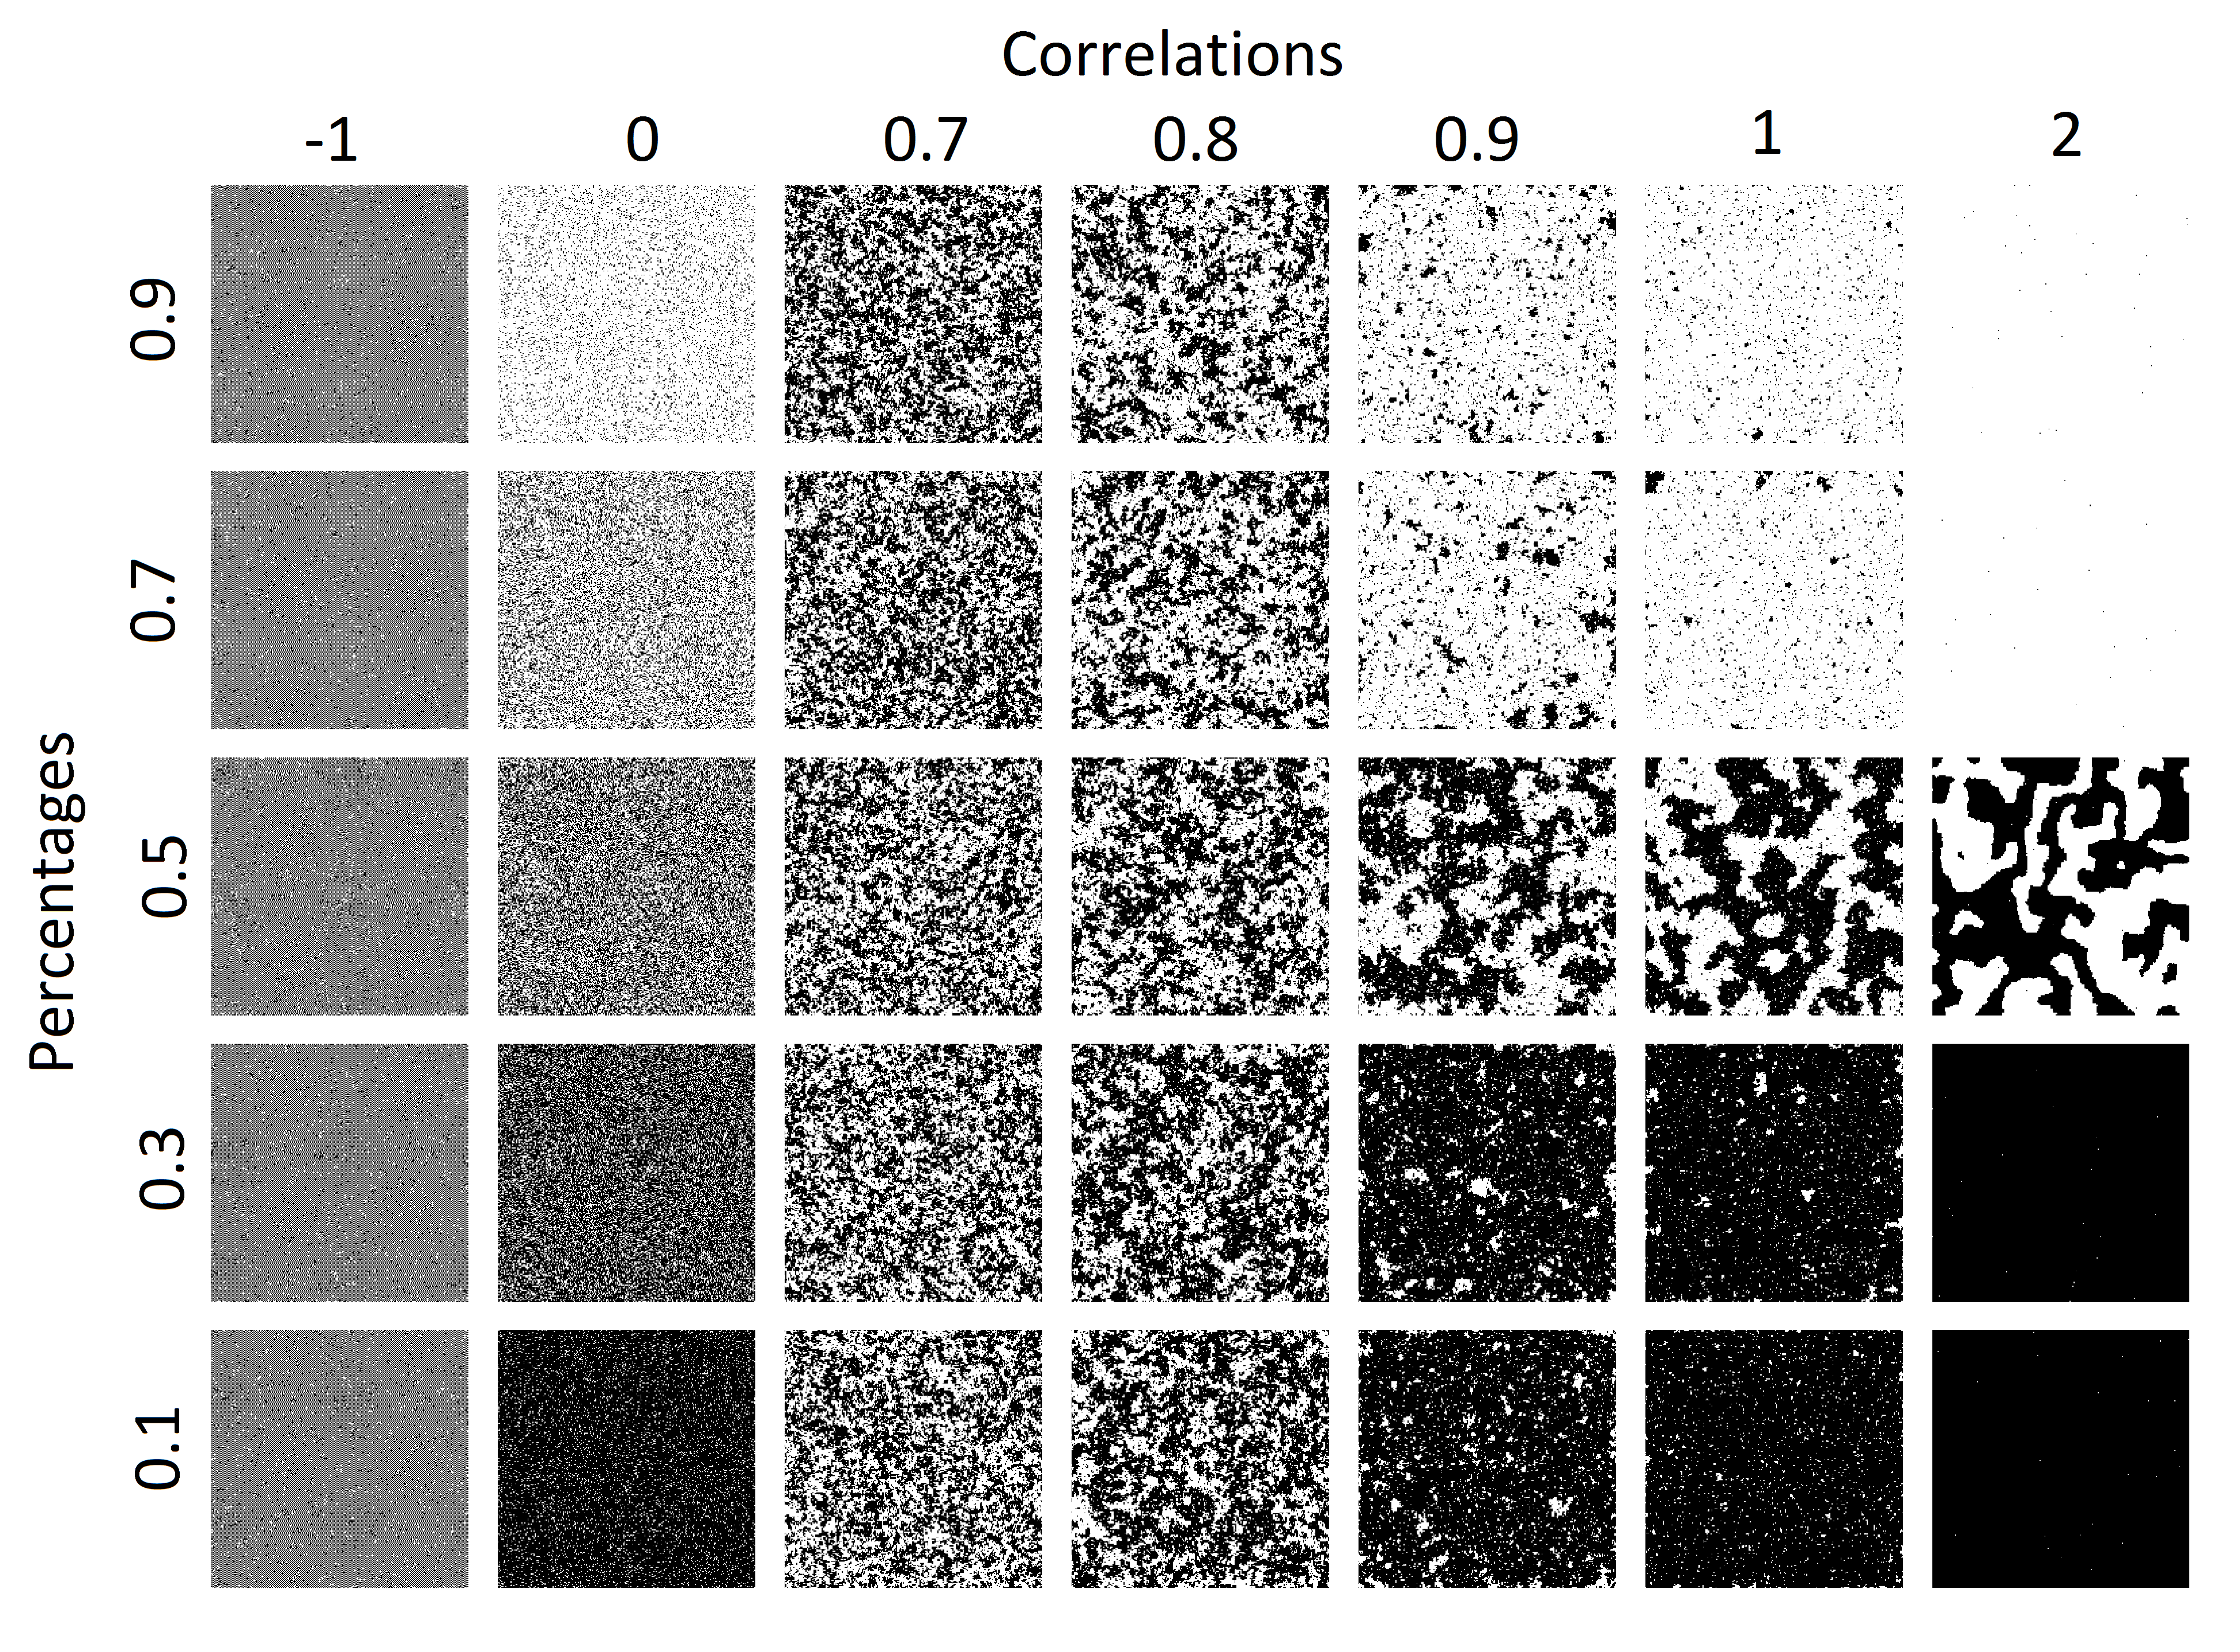
\includegraphics[scale=0.18]{gibbs_sampling}

        \caption{Final state of the grid after Gibbs sampling for different correlations and initial percentage of +1s}
        \label{figure:gibbs}
    \end{figure}
    
    The phase transition happens for a certain correlation between $0.8$ and $0.9$. Spins tend to align in a neighbourhood, and we observe a clear separation between +1 spins and -1 spins. For an initial population with high +1 percentage, all the grid aligns to +1 if the correlations between nodes is strong enough (equal to 2 in our tests).
    \\
    Interestingly though, for negative correlations, spins are completely random and we just observe noise, independently from the initial percentage of +1.
    
    \subsection{Mean field algorithm}
    Mean field is an iterative algorithm. Starting from a initial grid of mean parameters, the algorithm converges toward a state that minimizes the Kullback-Leibler divergence with respect to the true distribution $\mathrm{P}$.
    Interestingly, the mean field problem is non convex. The minimum can thus be a local minimum, in which the algorithm is stuck. Different initialization can yield different fixed points, as illustrated in figure \ref{figure:meanfieldconvprob} with $a=10$ and the potentials $b$ as plotted. The starting point 0 tends to give the expected result.
    
    \begin{figure}[h]
        \centering
        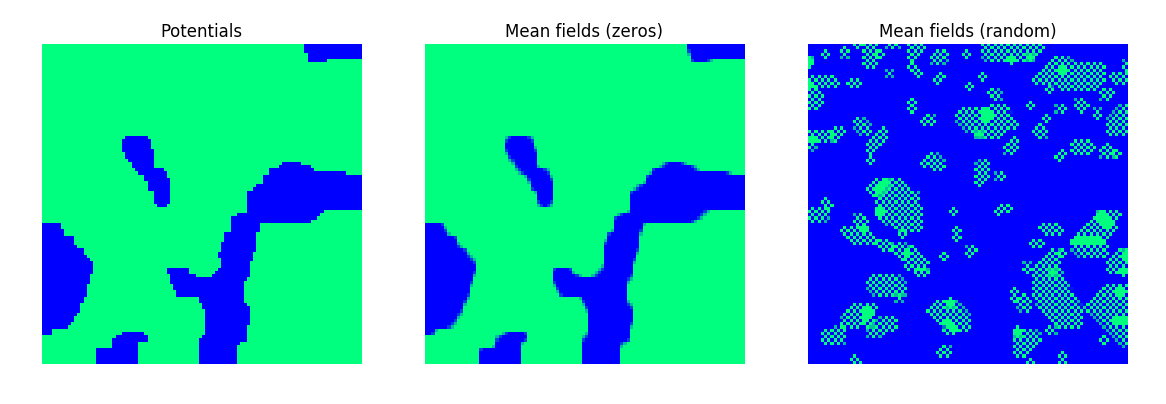
\includegraphics[width = 0.732\paperwidth]{meanfield_qui_chie_a10}
        \caption{Convergence of meanfield for different initializations. A random initialization converges to a local minimum. Starting from the grid mean value 0 (nodes take values \{-1, +1\} usually converges to the global minimum.}
        \label{figure:meanfieldconvprob}
    \end{figure}
    
    
    
    \subsection{Loopy belief algorithm}
    As we said earlier, loopy belief algorithm has no theoretical guarantee to work for graphs with cycles. Those very cycles, if not dealt with carefully, will just drive the messages to quickly diverge. Computational tricks should be used in the case of graphs with cycles, among them the grid. 
    Before adding the damping to loopy belief, we observed a clear dependence of the result on the update order, as seen in figure \ref{figure:lbupdateorder}.
    
    \begin{figure}[h]
        \centering
        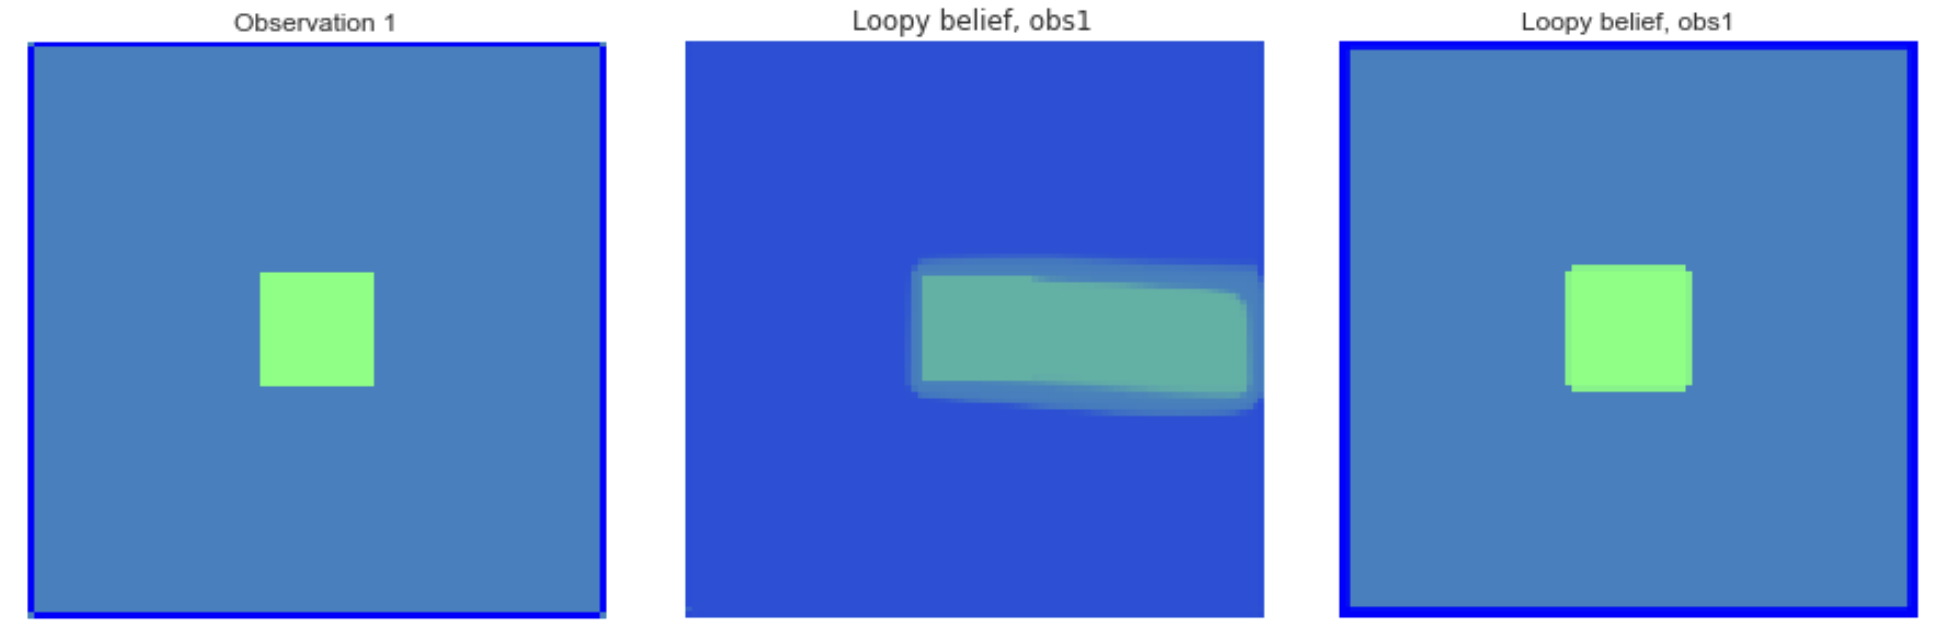
\includegraphics[width=0.72\paperwidth]{lb_before_damping}
        \caption{Loopy belief convergence for different update orders. The leftmost figure is the initial observation we have of the grid. Green is for +1, dark blue for -1, and turquoise for unobserved nodes (0). The figure in the center is obtained for a cyclic message update order, whereas the leftmost is obtained for a random message update order.}
        \label{figure:lbupdateorder}
    \end{figure}
    
    
    % Compare the algorithms to each other, for different observations,
    
    \subsection{Comparison of the 3 algorithms}
    Practically, we want to start from observed nodes and infer the rest of the distribution. This is what we implemented for mean field, loopy belief propagation and Gibbs sampling for 3 different observations. Figure \ref{figure:compare1} shows the different results obtained from the 3 algorithms as well as the 3 observations. In every case, $a=3$ and $b=0$.
    \\
    For each algorithm, the initial grid is the observation. 
    \\
    For loopy belief, the damping factor is $0.5$, and the update order is cyclic.
    \\
    For Gibbs sampling, we sample the grid 100 times for each observation, and then compute the mean grid to approximate to mean parameters.
    \begin{figure}[ht]
        \centering
    	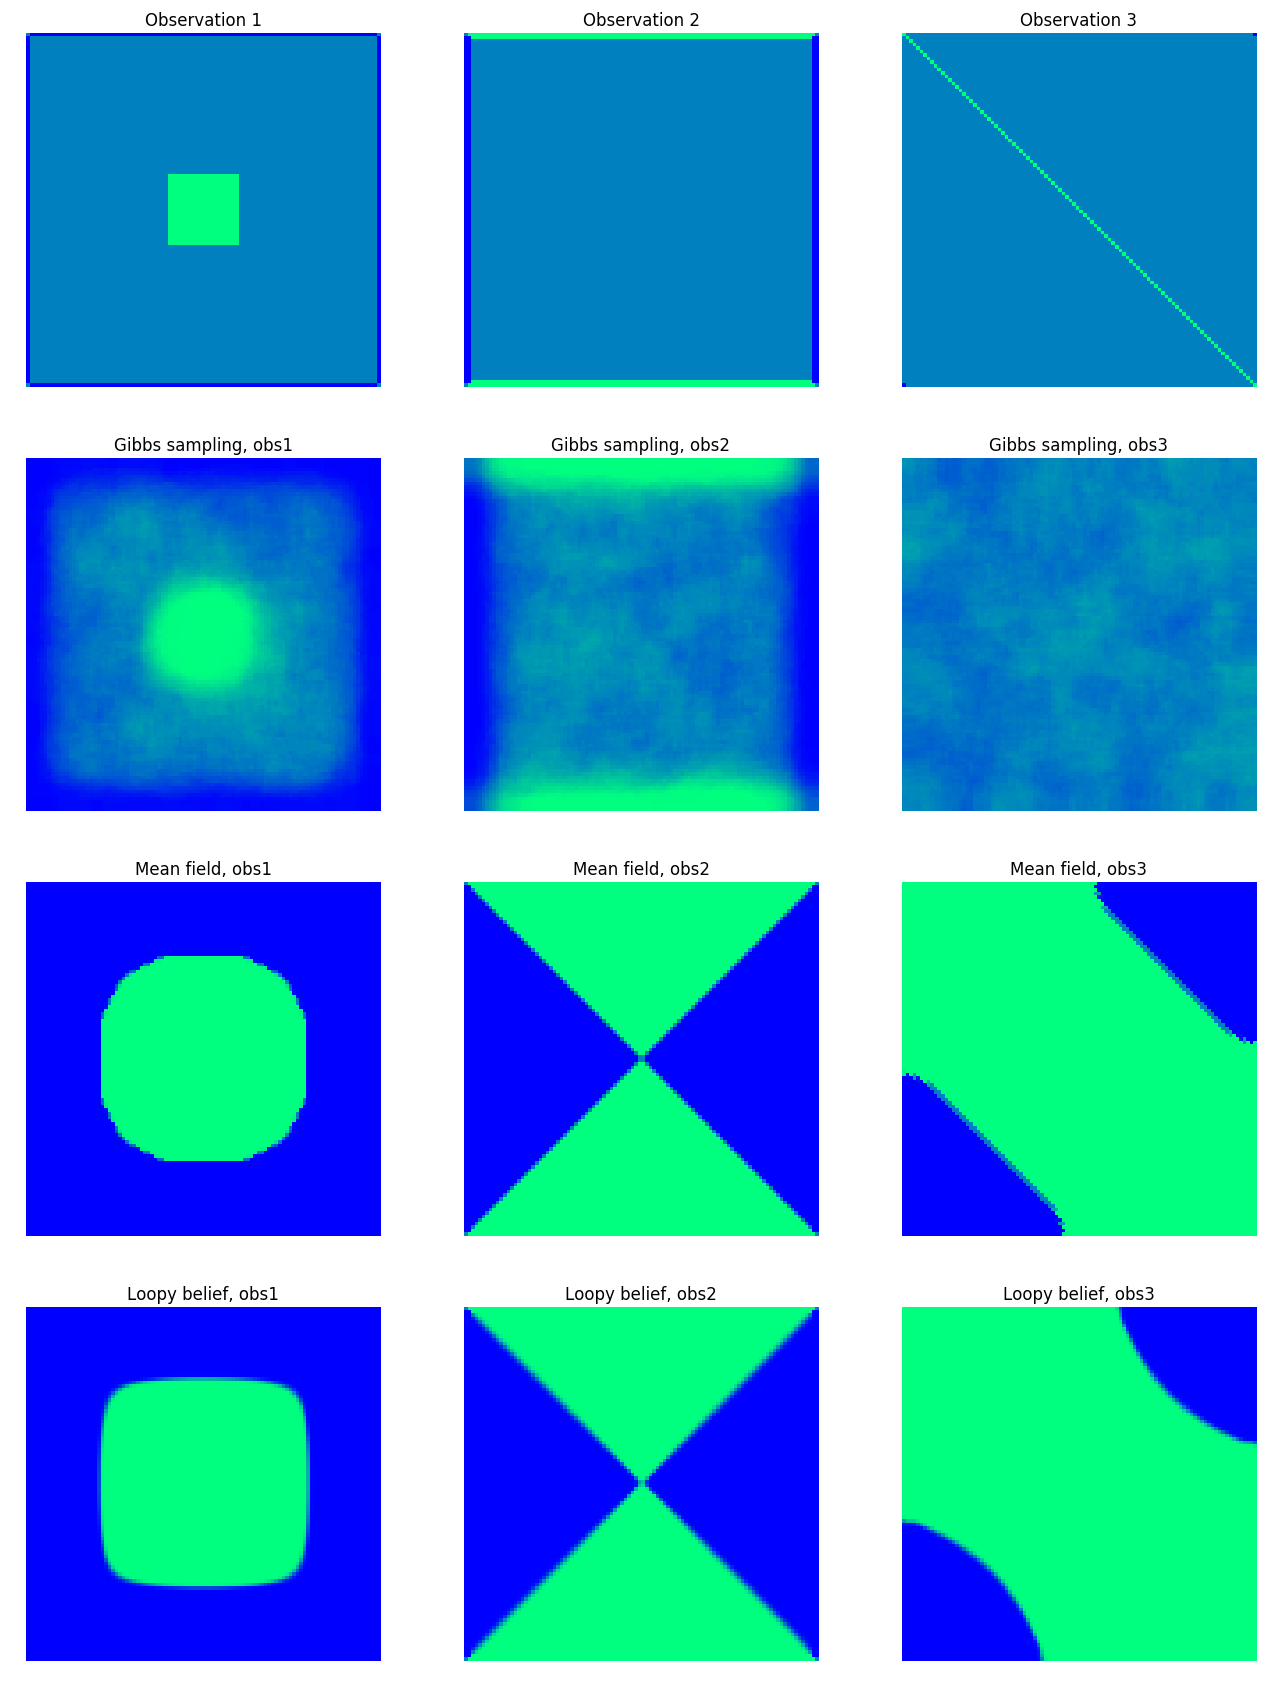
\includegraphics[scale=0.4]{compare_mf_lb_gibbs_3_3}
    	\caption{Mean parameters as computed by the 3 different algorithms for 3 different observations. The first row is for the observations. The second row is for the results of Gibbs sampling. The third row is for the results of mean field. The fourth row is for the results of loopy belief. All the algorithms were run on the same model of size $100 \times 100$, and with parameters $a=3$ and $b=0$.}
    	\label{figure:compare1}
    \end{figure}
    
    We also compared the convergence speed of the 3 algorithms for the same parameters. Figure \ref{figure:compare2} shows the energy evolution as a function of the iteration. Energies have been normalized first to fit the interval $[0,1]$ in order to allow for a valid comparison.
    
    \begin{figure}[ht]
        \centering
    	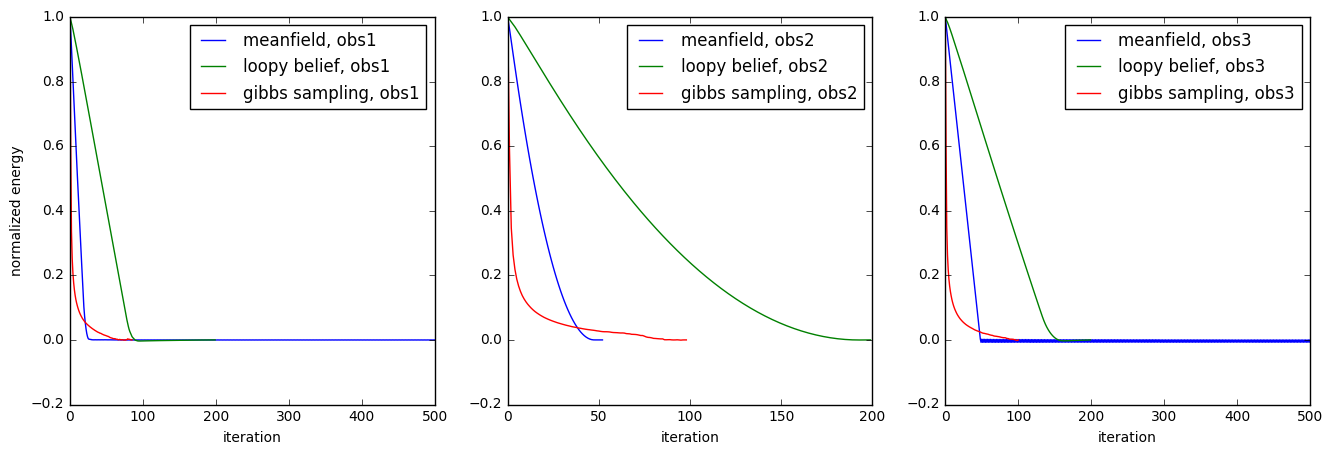
\includegraphics[width=0.72\paperwidth]{compare_mf_lb_gibbs_3_3bis}
    	\caption{Comparison of convergence speed for the 3 observations}
    	\label{figure:compare2}
    \end{figure}
    % Compare converging speeds,
    
    It is very important not to forget that Gibbs sampling needs to be run multiple times ($100$ in our tests) in order to compute the empirical means, so one should multiply the convergence time of Gibbs sampling by 100 for the real computation time. On the other hand, one loopy belief iteration takes slightly more time than an iteration of Gibbs sampling or mean field.

\section{Conclusion}
    % conclude 
    Approximate inference algorithms are used in practice for a variety of applications, even on trees or chains, for their efficiency and lower computation cost than exact inference algorithms. We've explored and tested 3 of these algorithms, each having its pros and cons. Gibbs sampling remains a sampling algorithm on the original problem, and thus the estimated mean parameters are estimated using the empirical mean of several observations. The mean field algorithm directly infers the mean parameters, but on a simpler graphical models (without the edges). This allows for a much lower computation time, but lower accuracy. Finally, Loopy belief algorithm estimates the mean parameters on the original graphical model, but is slower and has no theoretical convergence guarantee on graphs with cycles, in addition to computing an approximate and not the true mean parameters.
    
    
\bibliographystyle{plain}
\bibliography{bilbi}

\end{document}
